% 《物理实验报告模板.tex》的共同版式；所有实验模板均载入本文件。
\documentclass[UTF8,a4paper,10pt,fontset=fandol]{ctexart}
\usepackage[left=3.175cm,right=3.175cm,top=2.54cm,bottom=2.54cm]{geometry}
\usepackage{graphicx,tikz,pgfplots,needspace,adjustbox,booktabs,fancyhdr,lastpage,amsmath,amssymb,array,tabularx,longtable}
\pgfplotsset{compat=1.18}
\setlength{\parindent}{0pt}
\setlength{\parskip}{2pt}
\setlength{\headheight}{18pt}
\linespread{1}
\newcommand{\SetField}[2]{\expandafter\def\csname reportfield@#1\endcsname{#2}}
\makeatletter
\newcommand{\Field}[2][1.35cm]{%
  \ifcsname reportfield@#2\endcsname
    \expandafter\ifx\csname reportfield@#2\endcsname\@empty
      \underline{\makebox[#1]{\strut}}%
    \else\csname reportfield@#2\endcsname\fi
  \else\underline{\makebox[#1]{\strut}}\fi}
\makeatother
\newcommand{\MathField}[2][1.35cm]{%
  \ifcsname reportfield@math_#2\endcsname
    \csname reportfield@math_#2\endcsname
  \else\text{\Field[#1]{#2}}\fi}
\newcommand{\coverfield}[2]{%
  \noindent{\heiti\fontsize{18pt}{48pt}\selectfont
  \makebox[3.3cm][l]{#1}\underline{\makebox[8.8cm][c]{\Field[0pt]{#2}}}\par}}
\newcommand{\bindingline}[1][2.85]{%
  \begin{tikzpicture}[remember picture,overlay]
    \foreach \i in {0,...,38}{%
      \pgfmathsetmacro{\bindingy}{-#1-0.52*\i}%
      \ifnum\i=13\relax
        \node[inner sep=0pt] at ([xshift=1.05cm,yshift=\bindingy cm]current page.north west) {\songti\fontsize{10.5pt}{10.5pt}\selectfont 装};
      \else\ifnum\i=19\relax
        \node[inner sep=0pt] at ([xshift=1.05cm,yshift=\bindingy cm]current page.north west) {\songti\fontsize{10.5pt}{10.5pt}\selectfont 订};
      \else\ifnum\i=25\relax
        \node[inner sep=0pt] at ([xshift=1.05cm,yshift=\bindingy cm]current page.north west) {\songti\fontsize{10.5pt}{10.5pt}\selectfont 线};
      \else
        \pgfmathsetmacro{\bindingtop}{\bindingy+0.20}%
        \pgfmathsetmacro{\bindingbottom}{\bindingy-0.20}%
        \draw[line width=0.35pt,dash pattern=on 1.2pt off 1.8pt]
          ([xshift=1.05cm,yshift=\bindingtop cm]current page.north west)
          -- ([xshift=1.05cm,yshift=\bindingbottom cm]current page.north west);
      \fi\fi\fi}
  \end{tikzpicture}%
}
% 装订线印在每一页正文和原始数据页，续页也沿用母模板样式。
\newif\ifreportbinding
\AddToHook{shipout/foreground}{\ifreportbinding\bindingline\fi}
\fancypagestyle{report}{\fancyhf{}\fancyfoot[C]{第\thepage 页\quad 共\pageref{LastPage}页}\renewcommand{\headrulewidth}{0.4pt}}
\fancypagestyle{record}{\fancyhf{}\fancyhead[C]{原始数据记录单}\fancyfoot[C]{第\thepage 页\quad 共\pageref{LastPage}页}\renewcommand{\headrulewidth}{0.4pt}}
\newcommand{\ReportCover}[1]{%
  \thispagestyle{empty}\vspace*{1.0cm}
  \begin{center}
    
\includegraphics[width=8.184cm]{tongji_logo.jpeg}\par
    {\bfseries\fontsize{18pt}{24pt}\selectfont TONGJI UNIVERSITY\par}
    \vspace{1.5cm}{\heiti\fontsize{36pt}{44pt}\selectfont 物理实验报告\par}
  \end{center}
  \vspace{1.5cm}
  \coverfield{实验名称}{experiment}
  \coverfield{学生姓名}{student}
  \coverfield{学\hspace{1em}号}{student_id}
  \coverfield{组\hspace{1em}号}{group}
  \coverfield{实验日期}{date}
  \clearpage\reportbindingtrue\pagestyle{report}
  \begin{center}{\heiti\fontsize{14pt}{40pt}\selectfont #1\par}\end{center}}
\newcommand{\ReportSection}[1]{\Needspace{4\baselineskip}\par\vspace{0.35\baselineskip}{\heiti #1}\par}
\newcommand{\ReportSubsection}[1]{\Needspace{3\baselineskip}\par\vspace{0.2\baselineskip}{\bfseries #1}\par}
\newcommand{\ReportRecord}{%
  \clearpage\thispagestyle{record}
  \vspace*{0.6cm}（请将教师签字的实验数据记录单完整拍照粘贴至此处。）
}

% ===== 数据输入区开始 =====
\SetField{experiment}{透镜焦距的测量}
% 后端以 \SetField{字段名}{值} 填入数据；缺省值保持空白。
% 母模板封面字段：\Field{experiment} \Field{student} \Field{student_id} \Field{group} \Field{date}
% ===== 数据输入区结束 =====
\begin{document}\fontsize{10.5pt}{20pt}\selectfont
\ReportCover{透镜焦距的测量}
\ReportSection{实验目的}
1. 理解薄透镜成像公式及实物、虚物的物距符号，掌握四种焦距测量方法。\par
2. 用物像距法、共轭法和自准直法分别测凸透镜焦距，再用辅助成像测凹透镜焦距。\par
3. 比较方法间的一致性，识别光轴未对准、清晰像判断和透镜厚度带来的误差。\par
\ReportSection{实验原理}
薄透镜近轴成像满足 $\frac1u+\frac1v=\frac1f$；物像距法由 $f=\frac{uv}{u+v}$ 求焦距。共轭法固定物屏间距 $L>4f$，两次清晰成像的透镜位置差为 $D$，故 $f=\frac{L^2-D^2}{4L}$。自准直法借助平面镜使返回像与物重合，此时物位于透镜焦平面。对凹透镜，先用凸透镜形成虚物，再按符号约定使用 $u<0$、$v>0$；若分母接近零，结果会对位置误差十分敏感。
\begin{center}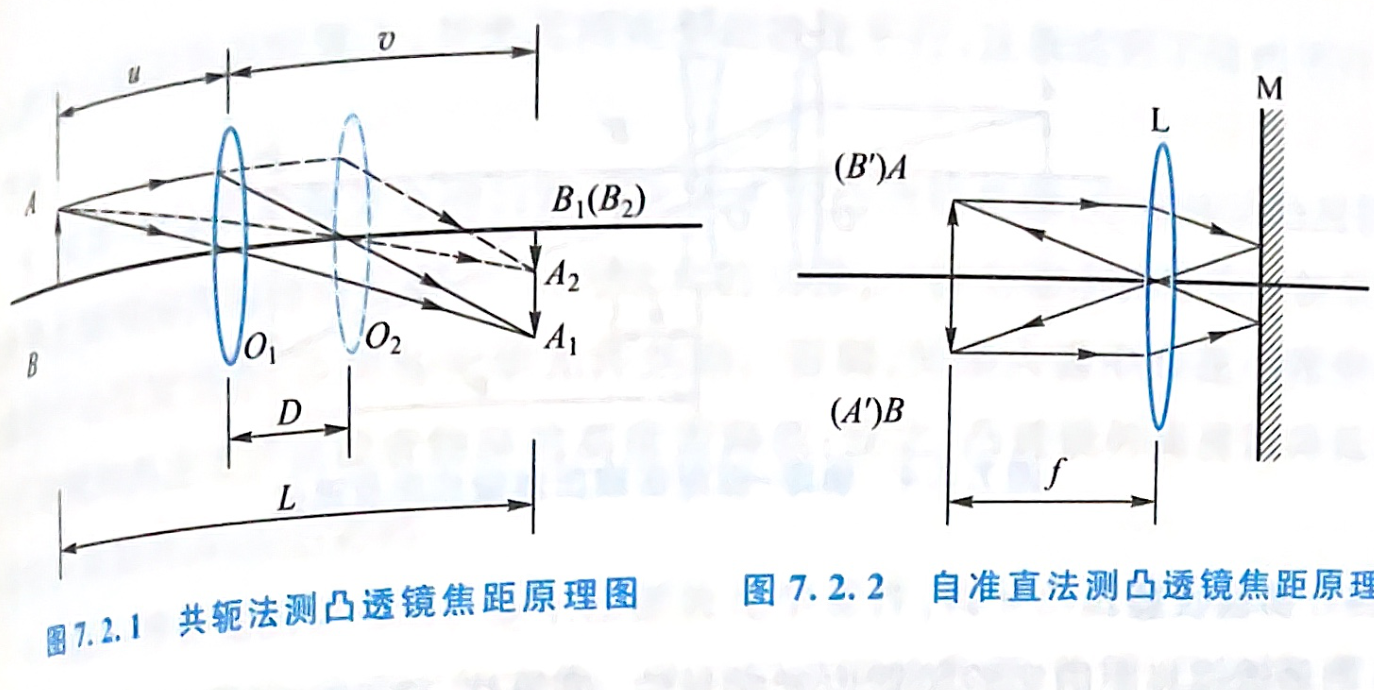
\includegraphics[width=10.3cm]{figures/lens-ray-diagrams.png}\par
{\small 共轭与自准直光路示意图。}\end{center}
\ReportSection{实验内容}
\ReportSubsection{调节与凸透镜测量}
1. 调整光源、透镜中心及屏幕中心共轴，记录各滑座位置时统一从同一刻线读取。\par
2. 物像距法测三组清晰像的物距与像距；共轭法固定五组物屏间距，在两清晰像位置测透镜位移；自准直法逐次调节平面镜使返回像与物重合，记录五组位置。\par
\ReportSubsection{凹透镜辅助成像}
3. 先用凸透镜形成实像，将凹透镜插在会聚光束中使该像成为凹透镜的虚物，再移动屏幕取得新的实像。\par
4. 对每组记录虚物、凹透镜及新像的位置；按统一的正负号计算凹透镜焦距，并检查五组结果的离散程度。
\ReportSection{实验仪器}
光学导轨、光源与物屏、凸透镜、凹透镜、平面镜及滑座。所有位置和距离输入均为 mm，混用 cm 会使报告结果错误。
\ReportSection{数据记录处理}
单次成像（mm）：
\begin{center}\small\renewcommand{\arraystretch}{1.35}
\begin{tabular}{|c|c|c|c|}\hline
次数 & $u$ & $v$ & $f$\\\hline
1 & \Field[10mm]{object_distance_01} & \Field[10mm]{image_distance_01} & \Field[10mm]{single_focus_01}\\\hline
2 & \Field[10mm]{object_distance_02} & \Field[10mm]{image_distance_02} & \Field[10mm]{single_focus_02}\\\hline
3 & \Field[10mm]{object_distance_03} & \Field[10mm]{image_distance_03} & \Field[10mm]{single_focus_03}\\\hline
\end{tabular}
\end{center}
\noindent 共轭法（mm）：
\begin{center}\small\renewcommand{\arraystretch}{1.35}
\begin{tabular}{|c|c|c|c|}\hline
次数 & $L$ & $D$ & $f$\\\hline
1 & \Field[10mm]{bessel_length_01} & \Field[10mm]{bessel_separation_01} & \Field[10mm]{bessel_focus_01}\\\hline
2 & \Field[10mm]{bessel_length_02} & \Field[10mm]{bessel_separation_02} & \Field[10mm]{bessel_focus_02}\\\hline
3 & \Field[10mm]{bessel_length_03} & \Field[10mm]{bessel_separation_03} & \Field[10mm]{bessel_focus_03}\\\hline
4 & \Field[10mm]{bessel_length_04} & \Field[10mm]{bessel_separation_04} & \Field[10mm]{bessel_focus_04}\\\hline
5 & \Field[10mm]{bessel_length_05} & \Field[10mm]{bessel_separation_05} & \Field[10mm]{bessel_focus_05}\\\hline
\end{tabular}
\end{center}
\noindent 自准直法（位置读数，mm）：
\begin{center}\small\renewcommand{\arraystretch}{1.35}
\begin{tabular}{|c|c|c|c|}\hline
次数 & 物位 & 凸透镜位 & $f$\\\hline
1 & \Field[10mm]{auto_object_01} & \Field[10mm]{auto_lens_01} & \Field[10mm]{auto_focus_01}\\\hline
2 & \Field[10mm]{auto_object_02} & \Field[10mm]{auto_lens_02} & \Field[10mm]{auto_focus_02}\\\hline
3 & \Field[10mm]{auto_object_03} & \Field[10mm]{auto_lens_03} & \Field[10mm]{auto_focus_03}\\\hline
4 & \Field[10mm]{auto_object_04} & \Field[10mm]{auto_lens_04} & \Field[10mm]{auto_focus_04}\\\hline
5 & \Field[10mm]{auto_object_05} & \Field[10mm]{auto_lens_05} & \Field[10mm]{auto_focus_05}\\\hline
\end{tabular}
\end{center}
\ReportSection{凹透镜辅助成像}
\noindent 凹透镜辅助成像（位置读数，mm）：
\begin{center}\small\renewcommand{\arraystretch}{1.35}
\begin{tabular}{|c|c|c|c|c|}\hline
次数 & 虚物位 & 凹透镜位 & 像位 & $f$\\\hline
1 & \Field[10mm]{concave_object_01} & \Field[10mm]{concave_lens_01} & \Field[10mm]{concave_image_01} & \Field[10mm]{concave_focus_01}\\\hline
2 & \Field[10mm]{concave_object_02} & \Field[10mm]{concave_lens_02} & \Field[10mm]{concave_image_02} & \Field[10mm]{concave_focus_02}\\\hline
3 & \Field[10mm]{concave_object_03} & \Field[10mm]{concave_lens_03} & \Field[10mm]{concave_image_03} & \Field[10mm]{concave_focus_03}\\\hline
4 & \Field[10mm]{concave_object_04} & \Field[10mm]{concave_lens_04} & \Field[10mm]{concave_image_04} & \Field[10mm]{concave_focus_04}\\\hline
5 & \Field[10mm]{concave_object_05} & \Field[10mm]{concave_lens_05} & \Field[10mm]{concave_image_05} & \Field[10mm]{concave_focus_05}\\\hline
\end{tabular}
\end{center}
\[\begin{aligned}
\bar f_{\rm single}&=(\MathField{focus_single_mean_mm}\pm\MathField{focus_single_u_mm})\,\mathrm{mm},\\
\bar f_{\rm Bessel}&=(\MathField{focus_bessel_mean_mm}\pm\MathField{focus_bessel_u_mm})\,\mathrm{mm},\\
\bar f_{\rm auto}&=(\MathField{focus_auto_mean_mm}\pm\MathField{focus_auto_u_mm})\,\mathrm{mm},\\
\bar f_{\rm concave}&=(\MathField{focus_concave_mean_mm}\pm\MathField{focus_concave_u_mm})\,\mathrm{mm}.
\end{aligned}\]
\noindent $u_f$ 为各方法重复测量的 A 类标准不确定度，未计入导轨读数和成像判断的系统误差。
\ReportSection{讨论与分析}
\ReportSubsection{各方法比较}
物像距法操作直观，但物距和像距都受清晰度判断影响；共轭法只需位置差，并应检查 $L>4f$；自准直法对返回像重合的判断较敏感。三法所得凸透镜焦距若明显不一致，应优先检查光轴共线和读数基准。\par
\ReportSubsection{凹透镜符号}
凹透镜的虚物位于透镜右侧，按本报告约定 $u=x_L-x_V<0$、$v=x_I-x_L>0$，由 $f=\frac{uv}{u+v}$ 得到负焦距。若把三个位置当作绝对距离代入，可能算出错误的正焦距。\par
\ReportSubsection{思考题}
为何共轭法要求 $L>4f$？否则不存在两个可区分的清晰成像透镜位置。为何应在导轨上反复检查共轴？偏轴会造成像差和读数误判。
\ReportSection{实验结论}
凸透镜焦距由物像距法、共轭法和自准直法分别得到 $\MathField{focus_single_mean_mm}$、$\MathField{focus_bessel_mean_mm}$、$\MathField{focus_auto_mean_mm}\,\mathrm{mm}$；辅助成像得到凹透镜焦距 $\MathField{focus_concave_mean_mm}\,\mathrm{mm}$。各值的重复测量标准不确定度见上式；结果需结合三法一致性与符号约定评价。

\ReportRecord
% ===== 原始数据图片插入区 =====
\end{document}
